\documentclass{article}
\usepackage{geometry}
\usepackage{subcaption}
\usepackage{parskip}
\usepackage{graphicx}
\usepackage{pythonhighlight}
\usepackage{amsmath}
\usepackage{hyperref}
\usepackage{float}
\makeatletter
\renewcommand\paragraph{\@startsection{paragraph}{4}{\z@}%
% display heading, like subsubsection
                                     {-3.25ex\@plus -1ex \@minus -.2ex}%
                                     {1.5ex \@plus .2ex}%
                                     {\normalfont\normalsize\bfseries}}
 \setcounter{secnumdepth}{4}
\makeatother
\newcommand{\code}[1]{\texttt{#1}}

\geometry{
  a4paper,
  margin=1in
}

\title{NLarge your dataset: Data augmentation for NLP}

\author{
  Ng Tze Kean \\
  \texttt{ngtzekean@gmail.com}
  \and
  Dexter Gui \\
  \texttt{dexter@email.com}
}

\begin{document}

\begin{titlepage}
  \centering
  
\includegraphics[width=1\textwidth]{img/ntu_logo.jpg}\par\vspace{1cm}
  \vspace{1.5cm}
  {\huge\bfseries NLarge your dataset: Data augmentation for NLP\par}
  \vspace{0.5cm}
  {\large NTU SC4002 Sem 1 2024\par}
  \vspace{2cm}
  \begin{minipage}[t]{0.45\textwidth}
    \centering
    {\Large Ng Tze Kean\par}
    \texttt{ngtzekean@gmail.com}
  \end{minipage}
  \hfill
  \begin{minipage}[t]{0.45\textwidth}
    \centering
    {\Large Dexter Gui\par}
    \texttt{dexter@email.com}
  \end{minipage}
  \vfill
  \today
\end{titlepage}

\begin{abstract}

  In this report, we explore the application of data augmentation (DA) techniques
  for Natural Language Processing (NLP) using a variety of methods including
  Large Language Models (LLMs). We demonstrate the effectiveness of these
  techniques in enhancing the diversity and robustness of the training data,
  potentially improving the performance of NLP models. We present our
  methodology, experimental results, and discuss the implications of our
  findings.

  Overall, we found that use of statistical methods such as substitution for data
  augmentation has limited applications. The use of more advanced deep learning
  models such as RNN with attention mechanisms tend to perform better in this
  task. The best results were obtained using Large Language Models (LLMs) for DA,
  which significantly improved the performance of the model.

\end{abstract}

\section{Introduction}

DA is a widely used technique in machine learning to enhance the diversity and
robustness of training datasets. By artificially expanding the dataset, DA
helps improve the generalization capabilities of models, particularly in
scenarios where labeled data is scarce or expensive to obtain
\cite{DBLP:journals/corr/abs-2105-03075}. In the context of Natural Language
Processing (NLP), DA poses unique challenges due to the complexity and
variability of human language.

Traditional DA methods in NLP, such as synonym replacement, random insertion,
and back-translation, have shown limited effectiveness in generating diverse
and meaningful variations of text data. These methods often fail to capture the
nuanced semantics and contextual dependencies inherent in natural language,
leading to suboptimal improvements in model performance.

Recent advancements in deep learning, particularly the development of Large
Language Models (LLMs) like GPT-2, GPT-3, and T5, have opened new avenues for
DA in NLP. These models, pre-trained on vast corpora of text data, possess a
remarkable ability to generate coherent and contextually relevant text.
Leveraging LLMs for DA involves generating synthetic data samples by providing
prompts based on existing training examples.

\subsection{Literature Review}

DA has been a widely researched area in the field of Natural Language
Processing (NLP) due to its potential to enhance the diversity and robustness
of training datasets \cite{DBLP:journals/corr/abs-2105-03075}. In the context
of sentiment analysis, DA techniques are particularly valuable as they help
improve the generalization capabilities of models, especially when labeled data
is scarce \cite{li-specia-2019-improving}.

Rule based methods like random replacement are quick to implement but lack the
generalisability to different corpus. These methods aim to generate new
training samples by making small perturbations to the existing data, thereby
increasing the size of the training set and improving the generalization
capabilities of sentiment analysis models \cite{wei-zou-2019-eda}.

Interpolation methods such as synonym replacement has also been developed
\cite{sahin-steedman-2018-data} where words in a sentence are replaced with
their synonyms. This method has been shown to improve model performance by
introducing lexical diversity. However, it often fails to capture the nuanced
semantics and contextual dependencies inherent in natural language, leading to
suboptimal improvements in sentiment analysis tasks
\cite{sahin-steedman-2018-data}.

Leading us to the current state of the art, the use of LLMs for data
augmentation has shown promising results in improving the performance of NLP
models \cite{ding-etal-2024-data}. By leveraging the generative capabilities of
LLMs we are able to reduce the amount of noise introduced and thus generate a
higher quality dataset. Most of the research has been focused on NER tasks, and
we aim to explore the feasibility of using LLMs for DA in sentiment analysis
tasks to ascertain the effectiveness of this approach.

Our hypothesis is that the benefits of LLM DA will still continue to provide
superior performance in sentiment analysis tasks over pre-LLM DA methods.

\subsection{Objective}

In this project, we explore the application of DA techniques for sentiment
analysis in NLP. We aim to evaluate the effectiveness of traditional DA methods
such as random substitution and synonym replacement, as well as advanced
techniques using LLMs for data augmentation.

The outcome would be a python library made open source with the implemented
methods and algorithms for the community to use.

\subsection{Training and Evaluation}

To evaluate the performance gain of the DA techniques, we augmented the dataset
at different levels: 5\%, 10\%, and 20\%. Afterwards, we will attempt extreme
cases of DA at 50\%, 100\%, and 200\% to observe the trend of the performance.

The base line model will be trained on the original dataset using a Recurrent
Neural Network (RNN) model to perform sentiment classification on the
validation dataset. We will then retrain the model using the augmented dataset
and compare the performance metrics to assess the impact of DA on model
performance.

We will also include a comparison of the performance of the RNN model with a
Long Short-Term Memory (LSTM) model to evaluate the impact of the model
architecture on the effectiveness of DA techniques.

\subsubsection{Model Architecture for Sentiment Classification}

The RNN model architecture consists of an embedding layer, followed by an RNN
layer, and a fully connected layer with a sigmoid activation function for
binary classification. The model was trained using the Adam optimizer with a
learning rate of \code{5e-4} and binary cross-entropy loss.

We adopted a pre-trained word embedding model to initialize the embedding layer
to transfer knowledge from the pre-trained model to our sentiment
classification task. The RNN layer uses a simple hidden layer our target is to
train that task layer to perform sentiment classification.

Our primary measure of improvement is the accuracy gain on the validation
dataset by the task specific RNN model. We also monitor the loss curves to
ensure that the model is not overfitting to the training data. Our hypothesis
is that the model will generalize better to unseen data with the augmented
dataset through various means to increase the volume of the corpus in
meaningful manners that will help the model learn and overfit less to the
training data.

\section{DA using Random Methods}

\subsection{Random Swap}

Let \( X = \{x_1, x_2, \ldots, x_n\} \) be a sequence of words in a text, where \( x_i \) represents the \( i \)-th word in the sequence.

The random swap process can be defined as follows:

For each word \( x_i \) in the sequence \( X \), with a probability \( p \), swap \( x_i \) with its adjacent word if \( x_i \) is not a stop word. Where \( x_j = x_{i+1} \) or \( x_j = x_{i-1} \).

\[
  x_i' =
  \begin{cases}
    \mathrm{swap}(x_i, x_j) & \mathrm{with\ probability\ } p \\
    x_i & \mathrm{with\ probability\ } 1 - p
  \end{cases}
\]

where \( x_i' \) is the new word after swap. The augmented sequence \( X' = \{x_1', x_2', \ldots, x_n'\} \) is then used as the new training sample.

The random swap process involves iterating over each word in the sequence and swapping with a predefined probability \( p \). This introduces variability into the dataset, potentially improving the robustness and generalization capabilities of NLP models.

\subsection{Random Substitution}

The random substitution process can be defined as follows:

For each word \( x_i \) in the sequence \( X \), with a probability \( p \), replace \( x_i \) with a randomly chosen word from the vocabulary \( V \).

\[
  x_i' =
  \begin{cases}
    \mathrm{random}(V) & \mathrm{with\ probability\ } p \\
    x_i & \mathrm{with\ probability\ } 1 - p
  \end{cases}
\]

where \( x_i' \) is the new word after substitution, and \( \mathrm{random}(V) \) denotes a randomly selected word from the vocabulary \( V \). The augmented sequence \( X' = \{x_1', x_2', \ldots, x_n'\} \) is then used as the new training sample.

The random substitution process introduces variability into the dataset by replacing words with random words from the vocabulary, potentially improving the robustness and generalization capabilities of NLP models.

\subsection{Random Deletion}

The random deletion process can be defined as follows:

For each word \( x_i \) in the sequence \( X \), with a probability \( p \), delete \( x_i \) from the sequence.

\[
  x_i' =
  \begin{cases}
    \emptyset & \mathrm{with\ probability\ } p \\
    x_i & \mathrm{with\ probability\ } 1 - p
  \end{cases}
\]

where \( x_i' \) is the new word after deletion, and \( \emptyset \) denotes the deletion of the word. The augmented sequence \( X' = \{x_1', x_2', \ldots, x_n'\} \) is then used as the new training sample.

The random deletion process introduces variability into the dataset by randomly removing words, potentially improving the robustness and generalization capabilities of NLP models.


\subsection{Results and Analysis}

To evaluate the effectiveness of random methods, we conducted experiments
with different levels of augmentation: 5\%, 10\%, and 20\% of the dataset. The
performance of the models trained with these augmented datasets was assessed
using accuracy score.

The results of our experiments indicate that the performance of the RNN model
keeps increasing with higher levels of augmentation. This suggests that data
augmentation provides a clear benefit for sentiment classification tasks.
Specifically, the model trained with 20\% augmented data achieved the highest
accuracy, followed by the models trained with 10\% and 5\% augmented data.
These findings highlight the importance of data augmentation in enhancing the
diversity and robustness of training datasets, leading to improved model
performance. We will report the results using random swap augmentation as we saw
no significant difference in the performance of the model using the different
random augmentation methods.

\begin{figure}[ht]
  \centering
  \begin{subfigure}[b]{0.3\textwidth}
    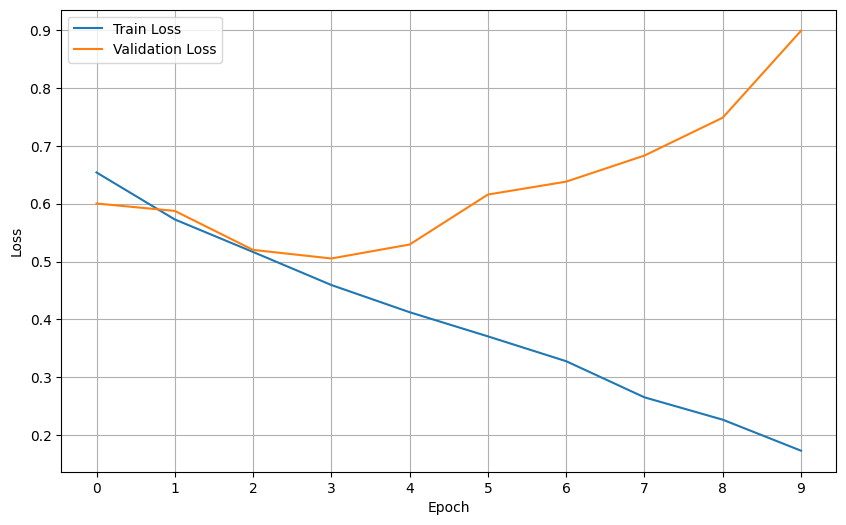
\includegraphics[width=\textwidth]{img/random_5.png}
    \caption{5\% Augmentation}
    \label{fig:random_5}
  \end{subfigure}
  \hfill
  \begin{subfigure}[b]{0.3\textwidth}
    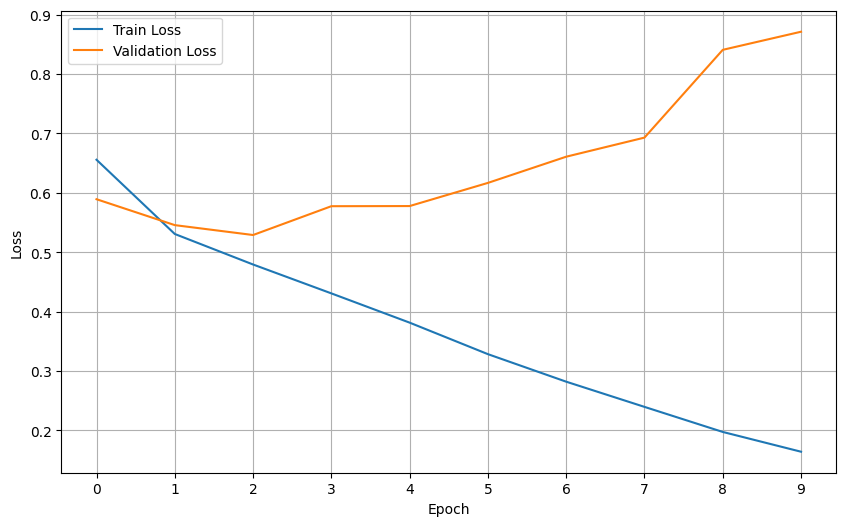
\includegraphics[width=\textwidth]{img/random_10.png}
    \caption{10\% Augmentation}
    \label{fig:random_10}
  \end{subfigure}
  \hfill
  \begin{subfigure}[b]{0.3\textwidth}
    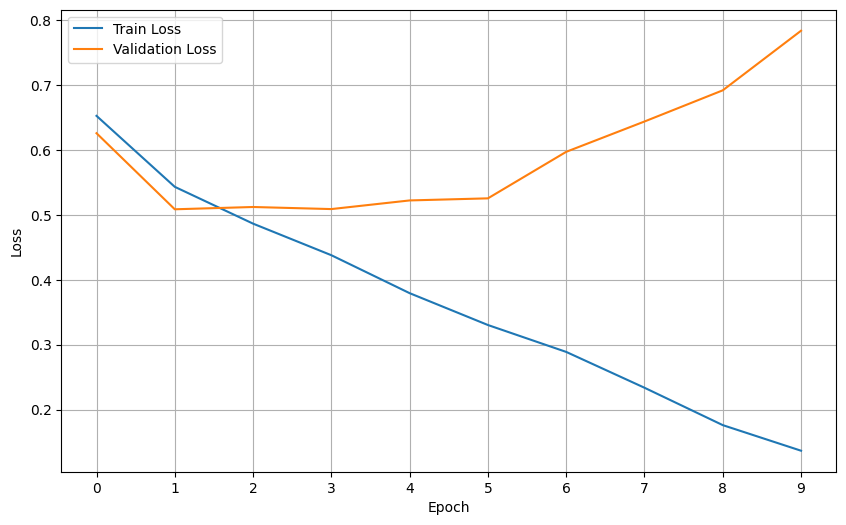
\includegraphics[width=\textwidth]{img/random_20.png}
    \caption{20\% Augmentation}
    \label{fig:random_20}
  \end{subfigure}
  \caption{Accuracy graphs for random augmentation DA at 5\%, 10\%, and 20\% levels.}
  \label{fig:random_substitution_acc}
\end{figure}

The observed trend, where the performance of the RNN model improves with higher
levels of data augmentation, can be attributed to several key factors. Firstly,
data augmentation techniques like random swap introduce increased data
diversity by exposing the model to a wider range of sentence
structures. This diversity helps the model learn more robust representations,
enhancing its ability to generalize to unseen examples.

Secondly, data augmentation mitigates over-fitting by effectively increasing
the size of the training dataset, reducing the likelihood of the model
memorizing specific examples and encouraging it to learn general patterns
instead. Additionally, the introduction of variations in the training data
makes the model more robust to noise and variations in real-world input data.
This robustness is crucial for achieving good performance on unseen data. An example
would be a change in the sentence structure from \code{I love this movie} to
\code{I movie this love}. which can help the model learn patterns that might be
found in the human speech patterns and thus generalize better on the test data.

Furthermore, data augmentation acts as a form of regularization, preventing the
model from becoming too complex and over-fitting the training data. By
providing a more comprehensive training dataset, data augmentation improves the
model's generalization capabilities, leading to better performance on
validation and test datasets. Collectively, these factors contribute to the
model's enhanced ability to learn effectively from the training data and
perform better on unseen examples.

\section{DA using Synonym Substitution}

In this subsection, we explore the performance of DA using synonym
substitution.

Let \( X = \{x_1, x_2, \ldots, x_n\} \) be a sequence of words in a text, where
\( x_i \) represents the \( i \)-th word in the sequence. Let \( S(x_i) \) be
the set of synonyms for the word \( x_i \).

The synonym substitution process can be defined as follows:

For each word \( x_i \) in the sequence \( X \), with a probability \( p \),
replace \( x_i \) with a randomly chosen synonym from \( S(x_i) \).
Mathematically, this can be expressed as:

\[
  x_i' =
  \begin{cases}
    \text{random}(S(x_i)) & \text{with probability } p     \\
    x_i                   & \text{with probability } 1 - p
  \end{cases}
\]

where \( x_i' \) is the new word after substitution, and
\(\text{random}(S(x_i))\) denotes a randomly selected synonym from the set \(
S(x_i) \).

The augmented sequence \( X' = \{x_1', x_2', \ldots, x_n'\} \) is then used as
the new training sample.

\subsection{Results and Analysis}

We can see from the results that generally as the augmentation level increases,
the performance of the model steadily increases as well.

% insert image 
\begin{figure}[ht]
  \centering
  \begin{subfigure}[b]{0.3\textwidth}
    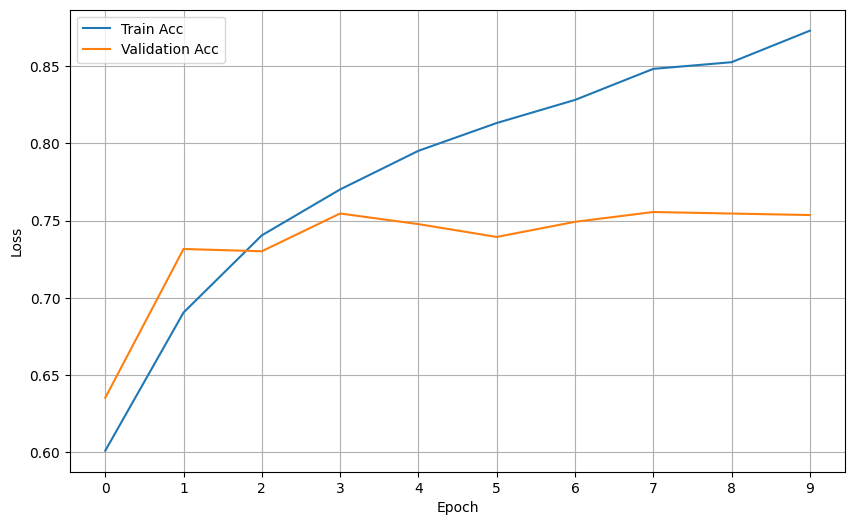
\includegraphics[width=\textwidth]{img/synonym_5.png}
    \caption{5\% Augmentation}
    \label{fig:synonym_5}
  \end{subfigure}
  \hfill
  \begin{subfigure}[b]{0.3\textwidth}
    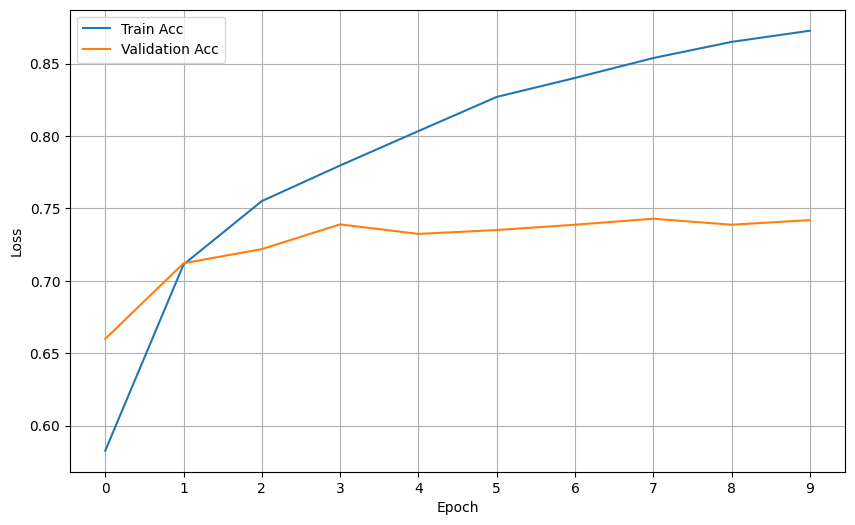
\includegraphics[width=\textwidth]{img/synonym_10.png}
    \caption{10\% Augmentation}
    \label{fig:synonym_10}
  \end{subfigure}
  \hfill
  \begin{subfigure}[b]{0.3\textwidth}
    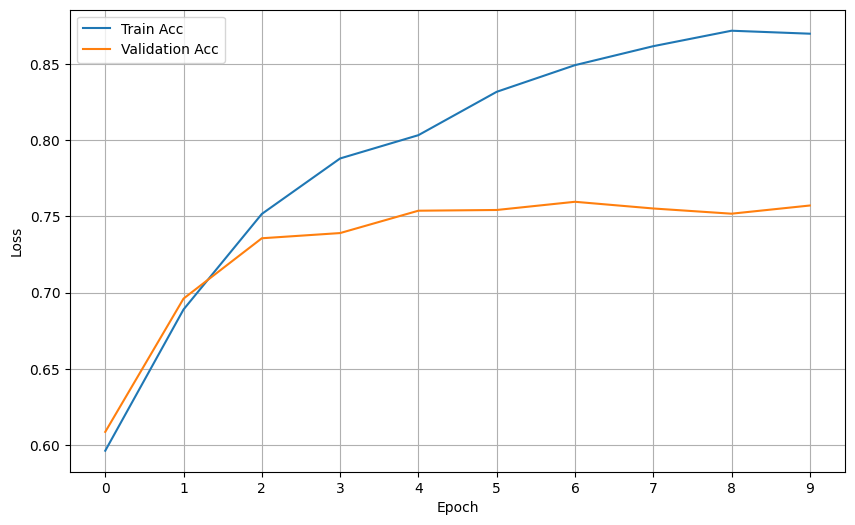
\includegraphics[width=\textwidth]{img/synonym_20.png}
    \caption{20\% Augmentation}
    \label{fig:synonym_20}
  \end{subfigure}
  \caption{Accuracy graphs for synonym augmentation DA at 5\%, 10\%, and 20\% levels.}
  \label{fig:synonym_substitution_acc}
\end{figure}

\section{Extreme DA}

We define extreme DA as augmentation past 50\% of the dataset. To explore the
trend of the performance, we augmented the dataset at 50\%, 100\% and 200\%
levels on each of the above methods and observed the performance of the model.

\subsection{Results and Analysis}

What is interesting is the continued improvement of the model. The RNN model
consistently improves with higher levels of augmentation. This suggests that
the RNN model is more robust to the increased data diversity introduced by
extreme DA (Figure \ref{fig:random_extreme_substitution_acc},
\ref{fig:synonym_extreme_substitution_acc}).

\begin{figure}[ht]
  \centering
  \begin{subfigure}[b]{0.3\textwidth}
    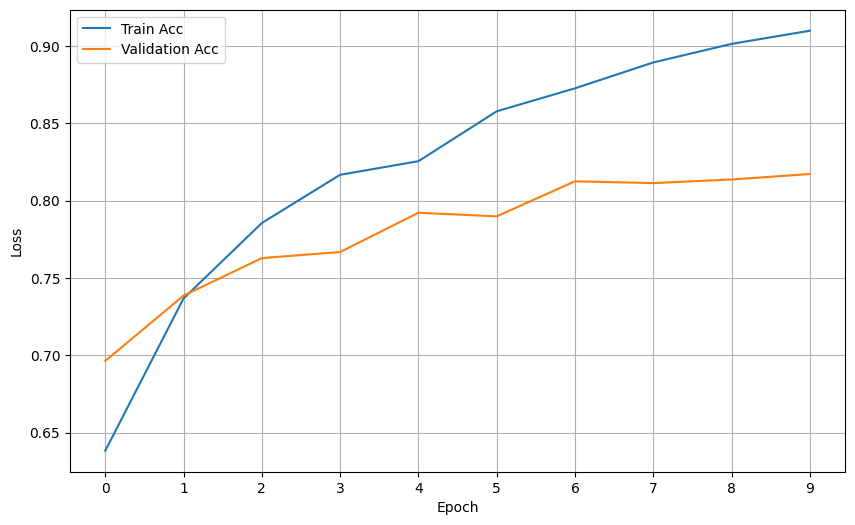
\includegraphics[width=\textwidth]{img/random_50.png}
    \caption{50\% Augmentation}
    \label{fig:random_50}
  \end{subfigure}
  \hfill
  \begin{subfigure}[b]{0.3\textwidth}
    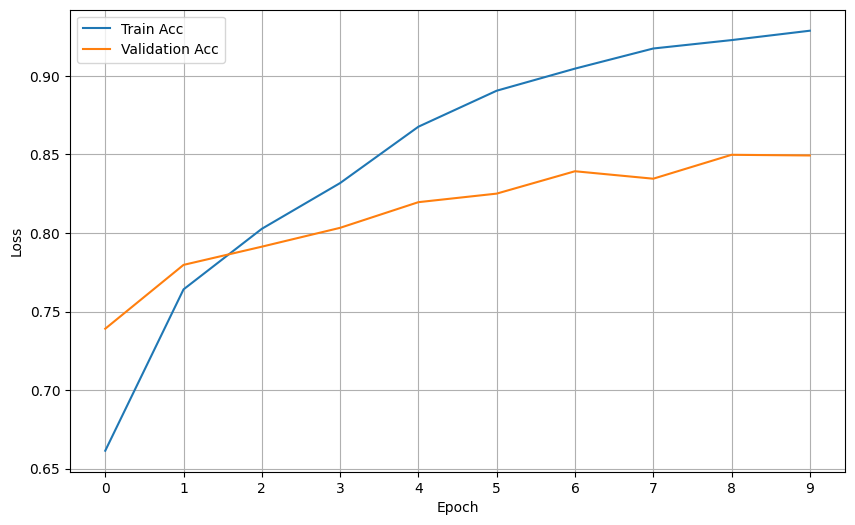
\includegraphics[width=\textwidth]{img/random_100.png}
    \caption{100\% Augmentation}
    \label{fig:random_100}
  \end{subfigure}
  \hfill
  \begin{subfigure}[b]{0.3\textwidth}
    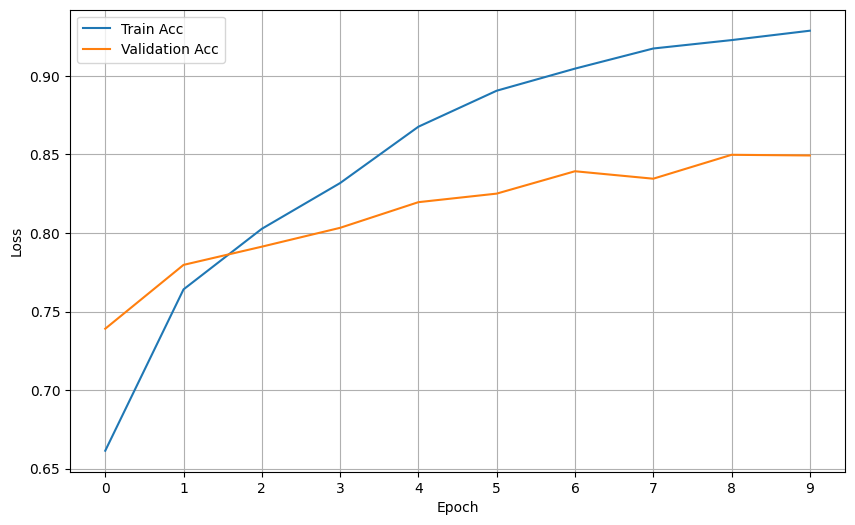
\includegraphics[width=\textwidth]{img/random_100.png}
    \caption{200\% Augmentation}
    \label{fig:random_100}
  \end{subfigure}
  \caption{Accuracy graphs for random augmentation DA at 50\%, 100\%, and 200\% levels.}
  \label{fig:random_extreme_substitution_acc}
\end{figure}

\begin{figure}[ht]
  \centering
  \begin{subfigure}[b]{0.3\textwidth}
    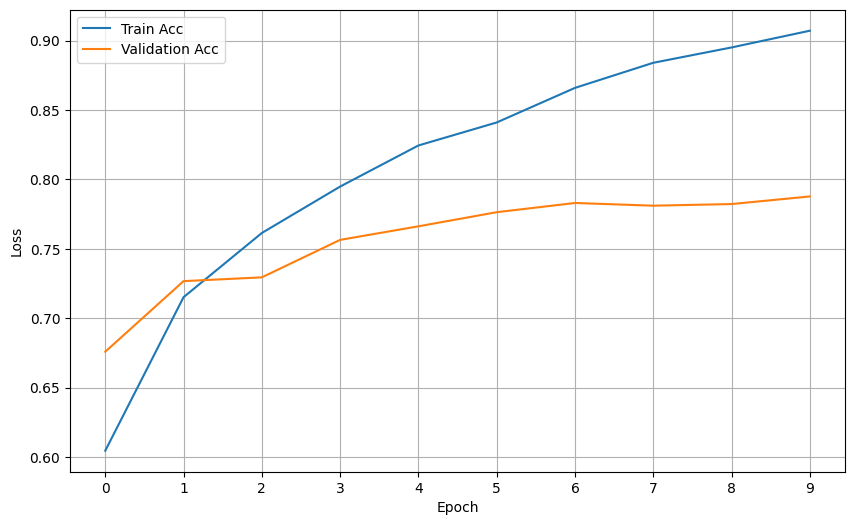
\includegraphics[width=\textwidth]{img/synonym_50.png}
    \caption{50\% Augmentation}
    \label{fig:synonym_50}
  \end{subfigure}
  \hfill
  \begin{subfigure}[b]{0.3\textwidth}
    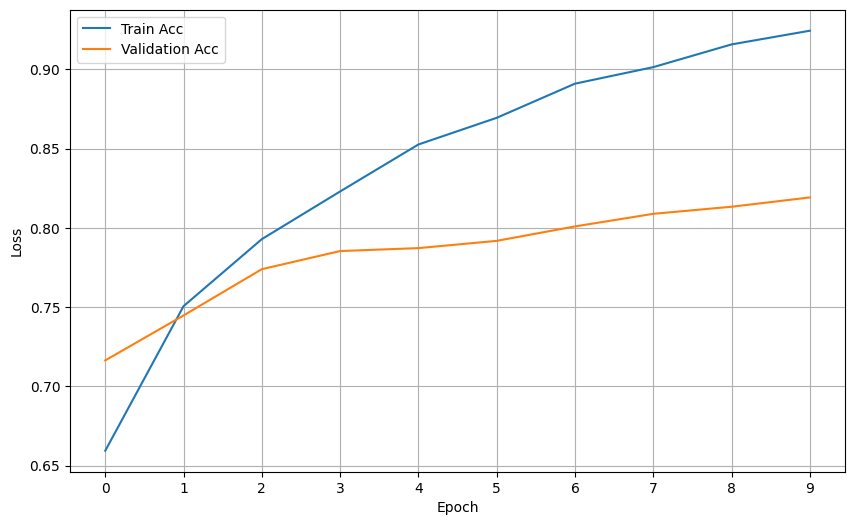
\includegraphics[width=\textwidth]{img/synonym_100.png}
    \caption{100\% Augmentation}
    \label{fig:synonym_100}
  \end{subfigure}
  \hfill
  \begin{subfigure}[b]{0.3\textwidth}
    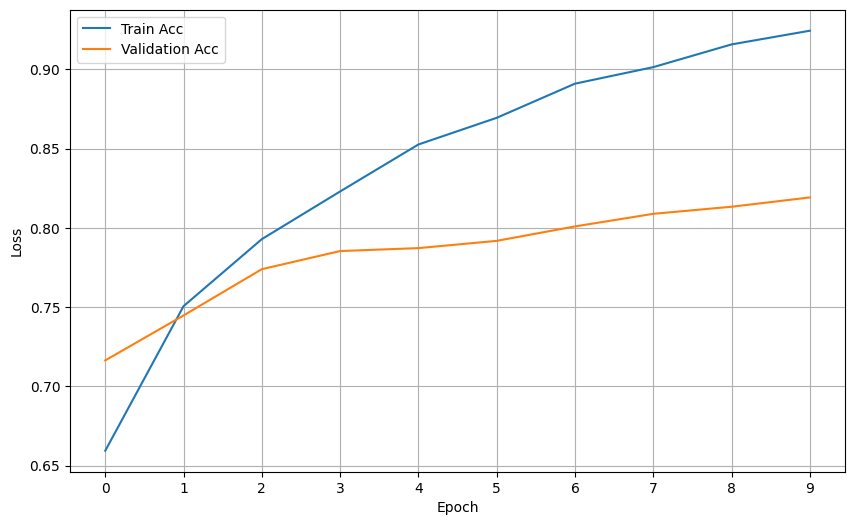
\includegraphics[width=\textwidth]{img/synonym_100.png}
    \caption{200\% Augmentation}
    \label{fig:synonym_100}
  \end{subfigure}
  \caption{Accuracy graphs for synonym augmentation DA at 50\%, 100\%, and 200\% levels.}
  \label{fig:synonym_extreme_substitution_acc}
\end{figure}

\section{DA using Hybrid (Synonym + Random) Substitution}

In light of the results from above, we are interested how the performance might
change in the case of a hybrid augmentation. We combined the synonym and random
and explored the changes in the performance of the model.

\subsection{Results and Analysis}

In general, when using the hybrid augmentation, the performance of the model
becomes more sporadic and not as consistent as using individual methods alone.
When a single method dominates the hybrid augmentation, such as a 100\% random
+ 50\% synonym approach, the performance of the model varies depending on the
seed used.

\begin{figure}[ht]
  \centering
  \begin{subfigure}[b]{0.45\textwidth}
    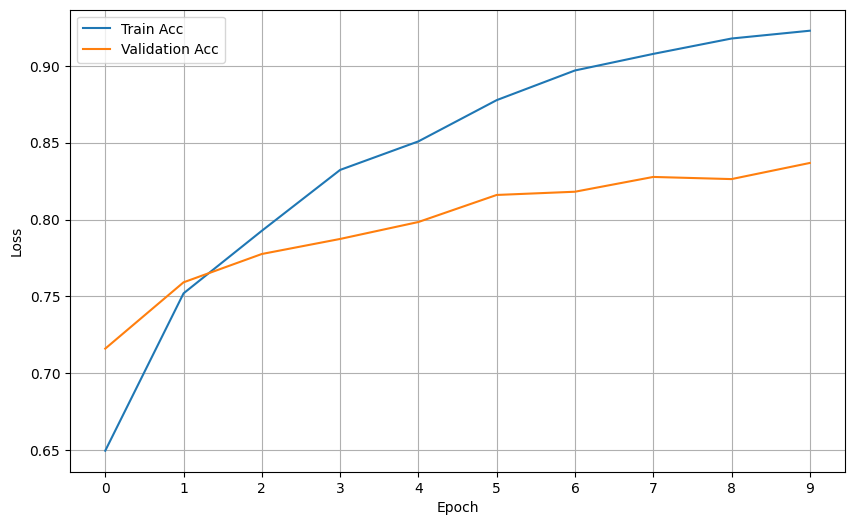
\includegraphics[width=\textwidth]{img/hybrid_100_rnn.png}
    \caption{50\% Random + 50\% Synonym Augmentation on RNN}
    \label{fig:hybrid_100_rnn}
  \end{subfigure}
  \hfill
  \begin{subfigure}[b]{0.45\textwidth}
    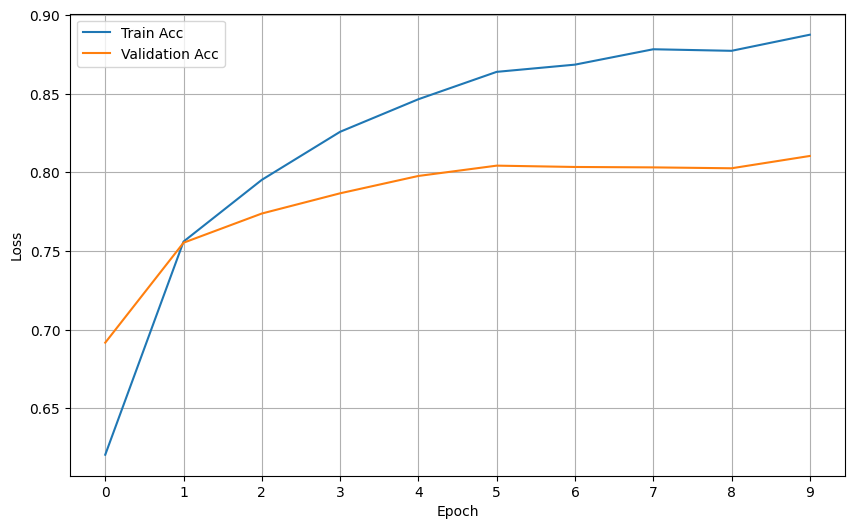
\includegraphics[width=\textwidth]{img/hybrid_100_lstm.png}
    \caption{50\% Random + 50\% Synonym Augmentation on LSTM}
    \label{fig:hybrid_100_lstm}
  \end{subfigure}
  \caption{Accuracy graphs for hybrid augmentation levels.}
  \label{fig:hybrid_extreme_substitution_acc_5050}
\end{figure}

It is worth noting that comparing both Figure
\ref{fig:hybrid_extreme_substitution_acc_2575} and
\ref{fig:hybrid_extreme_substitution_acc_100100} we can see that there little
performance gain. In other settings, the performance of the model is less
stable and takes more time for convergence.

\begin{figure}[ht]
  \centering
  \begin{subfigure}[b]{0.45\textwidth}
    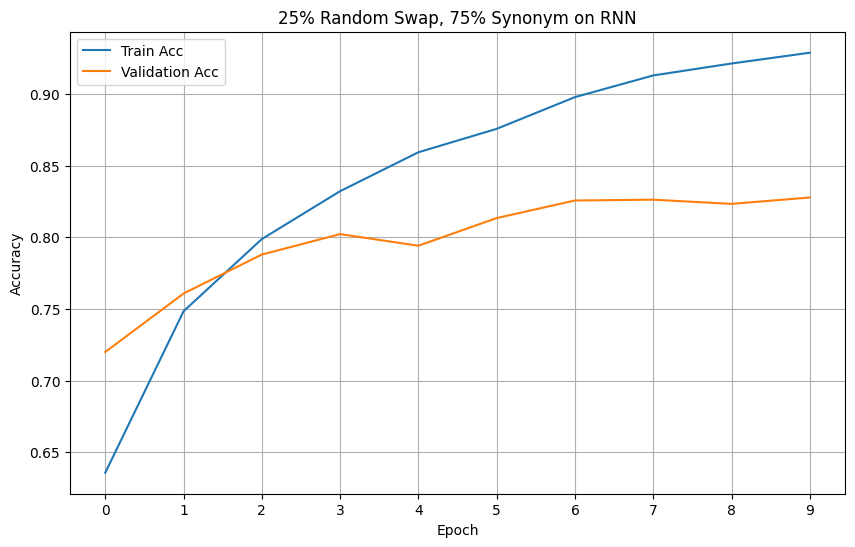
\includegraphics[width=\textwidth]{img/random_25_synonym_75_rnn.png}
    \caption{25\% Random + 75\% Synonym Augmentation on RNN}
    \label{fig:random_25_synonym_75_rnn}
  \end{subfigure}
  \hfill
  \begin{subfigure}[b]{0.45\textwidth}
    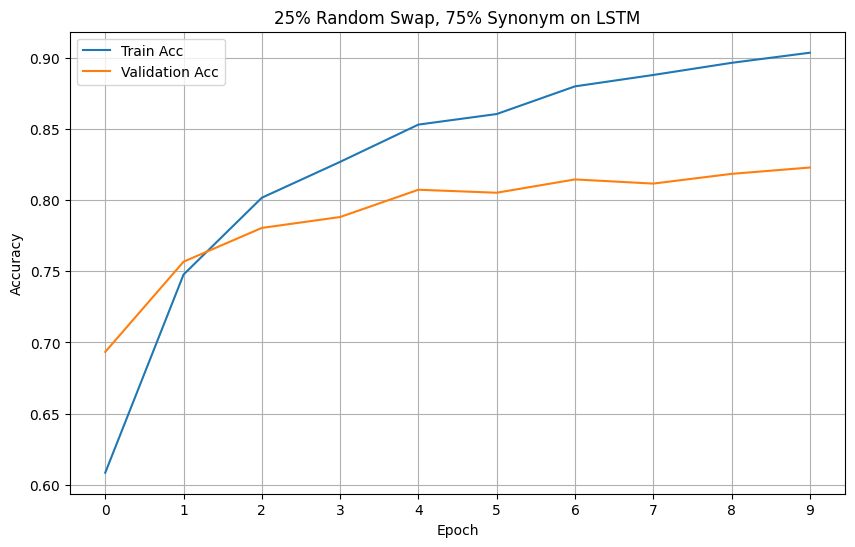
\includegraphics[width=\textwidth]{img/random_25_synonym_75_lstm.png}
    \caption{25\% Random + 75\% Synonym Augmentation on LSTM}
    \label{fig:random_25_synonym_75_lstm}
  \end{subfigure}
  \caption{Accuracy graphs for hybrid augmentation levels.}
  \label{fig:hybrid_extreme_substitution_acc_2575}
\end{figure}

\begin{figure}[H]
  \centering
  \begin{subfigure}[b]{0.45\textwidth}
    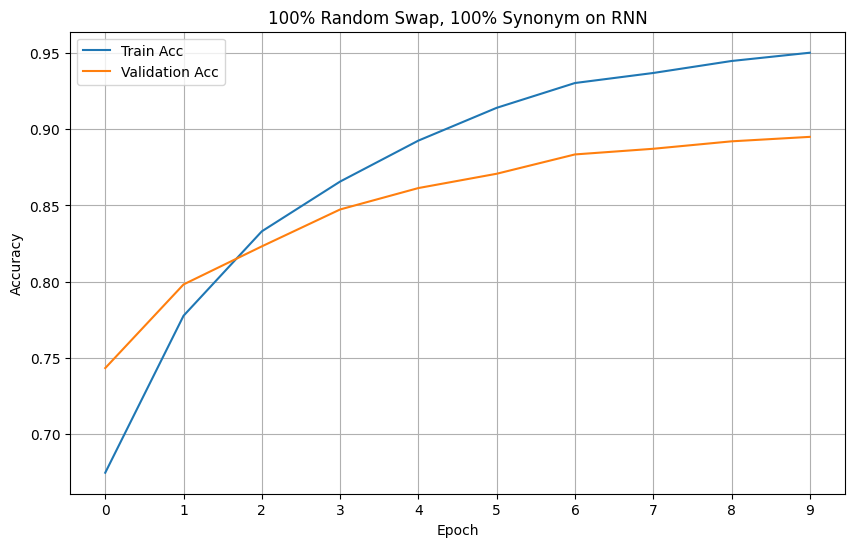
\includegraphics[width=\textwidth]{img/random_100_synonym_100_rnn.png}
    \caption{100\% Random + 100\% Synonym Augmentation on RNN}
    \label{fig:random_100_synonym_100_rnn}
  \end{subfigure}
  \hfill
  \begin{subfigure}[b]{0.45\textwidth}
    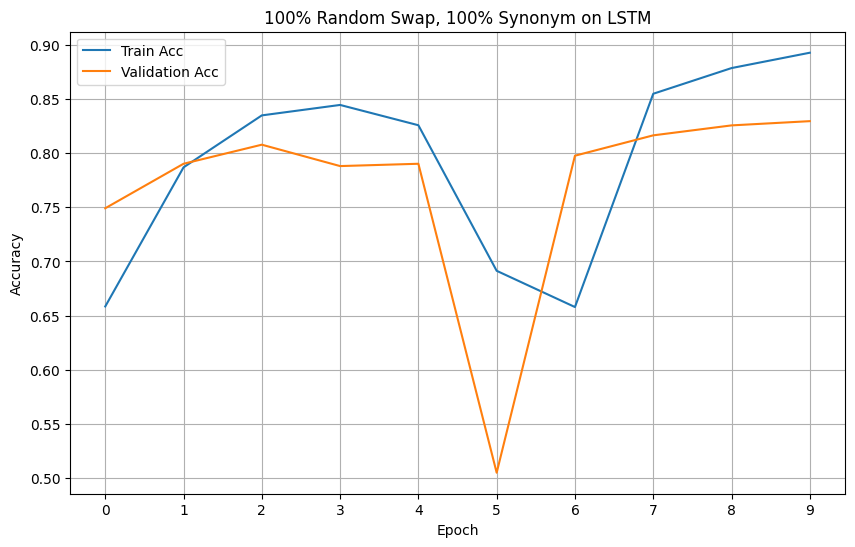
\includegraphics[width=\textwidth]{img/random_100_synonym_100_lstm.png}
    \caption{100\% Random + 100\% Synonym Augmentation on LSTM}
    \label{fig:random_100_synonym_100_lstm}
  \end{subfigure}
  \caption{Accuracy graphs for hybrid augmentation levels.}
  \label{fig:hybrid_extreme_substitution_acc_100100}
\end{figure}

This presents an interesting observation that mixing augmentation methods
togethers could instead cause degradation of performance or waste compute
resources when not tuned properly.

In light of this, we want to explore if the use of LLMs for DA could provide
better results.

\section{DA using LLMs}

To enhance the diversity and robustness of our dataset, we employed a data
augmentation technique leveraging pre-trained Large Language Models (LLM) from
the Transformers library.

Specifically, we utilized the model to generate synthetic data samples by
providing prompts based on existing training examples. We used types of
approach to generate the samples. The first is using a model through question
and answering to generate the samples. The second is to use a model that
performs summarization of content.

The summarizer was easy to implement as it generated relevant samples, however,
the question and answer technique was sporadic and often generated repeated
text. We will note some of challenges and solution that we applied in this
approach.

\subsubsection{LLM selection}

The choice of the model is crucial as it determines the quality of the
generated samples. We experimented with several models, including GPT-2, GPT-3,
and T5. As we tried to perform prompt engineering to generate diverse samples,
we found that these models could not adequately paraphrase the training data,
more often than not, producing the exact same text or slightly modified
versions of the original text.

We suspect that these LLM do not perform well due to the lack of contextual
information in the prompt. We hypothesize that the models require more
contextual information to generate diverse samples. We realized that a model
that allows us to specify a role for the prompt, we would be able to generate
more diverse samples.

\subsubsection{Prompt Engineering}

We proceeded to experiment with the Qwen model, with some of the techniques
applied from \cite{promptingguide}. We found that the Qwen model allows us to
specify a role for the prompt, which allows us to instruct the model to
specifically only paraphrase the verbs and structure of the sentence. This
allows us to generate a text that differs from the original text, while still
retaining the meaning of the original text.

\subsubsection{Results and Analysis}

\paragraph{Question and Answer Model}

We observed that with the Qwen model, we were able to generate diverse and
relevant samples, yet the performance of the model did not improve and in fact
there was degradation in the performance of the model. This can be seen from
Figure \ref{fig:llm_rnn_substitution_accuracy} and Table
\ref{table:rnn_performance}. This is very unexpected as we hypothesized that
the diverse samples would improve the performance of the model. Our hypothesis
that using a expert model to increase the diversity of the samples would
improve the performance of the model was not supported by the results.

\begin{figure}[ht]
  \centering
  \begin{subfigure}[b]{0.3\textwidth}
    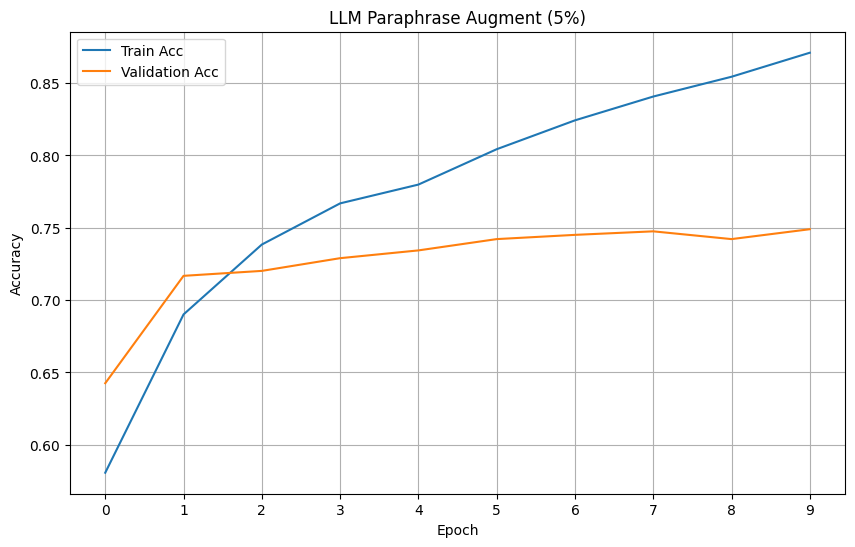
\includegraphics[width=\textwidth]{img/llm_5_rnn.png}
    \caption{5\% Augmentation}
    \label{fig:llm_5_rnn}
  \end{subfigure}
  \hfill
  \begin{subfigure}[b]{0.3\textwidth}
    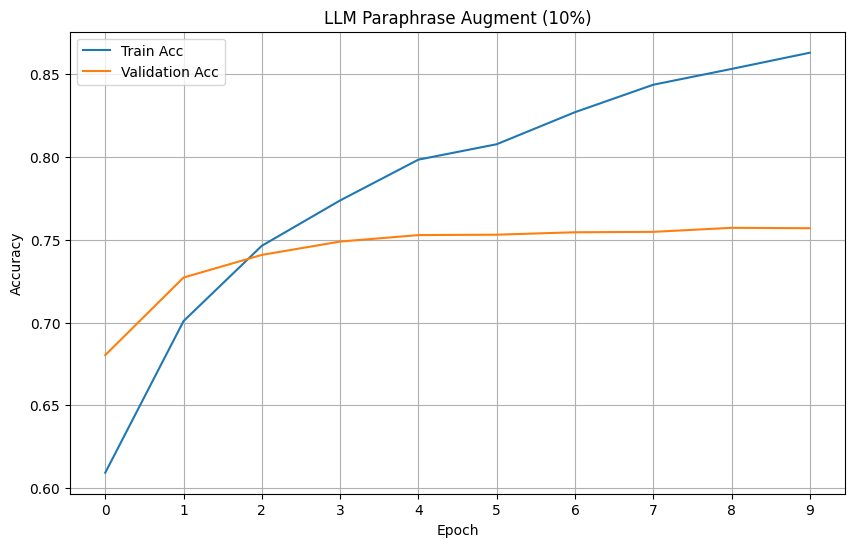
\includegraphics[width=\textwidth]{img/llm_10_rnn.png}
    \caption{10\% Augmentation}
    \label{fig:llm_10_rnn}
  \end{subfigure}
  \hfill
  \begin{subfigure}[b]{0.3\textwidth}
    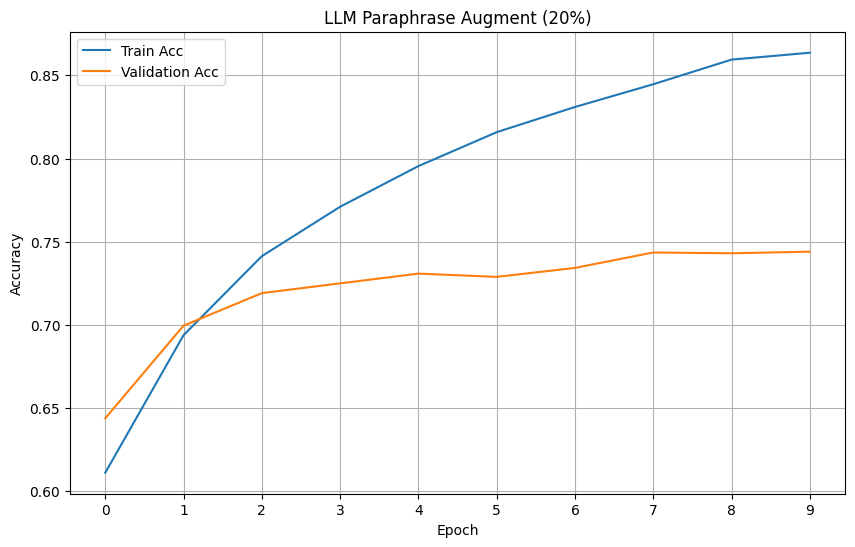
\includegraphics[width=\textwidth]{img/llm_20_rnn.png}
    \caption{20\% Augmentation}
    \label{fig:llm_20_rnn}
  \end{subfigure}
  \caption{Accuracy graphs for LLM substitution DA at 5\%, 10\%, and 20\% levels on RNN.}
  \label{fig:llm_rnn_substitution_accuracy}
\end{figure}

We examined the possible causes of this unexpected result and found that the
augmentation generated by the Qwen model was too long at 100 tokens that the
RNN suffered from vanishing gradients. We hypothesize that there was 2 main
issues:

\begin{enumerate}
  \item Vanishing gradients due to the long sequences generated
  \item RNN suffering from the long sequences generated
\end{enumerate}

\begin{table}[ht]
  \centering
  \begin{tabular}{|c|c|c|}
    \hline
    \textbf{Augmentation Level} & \textbf{Train Accuracy} & \textbf{Validation Accuracy} \\
    \hline
    5\%                         & 0.875                   & 0.751                        \\
    \hline
    10\%                        & 0.873                   & 0.757                        \\
    \hline
    20\%                        & 0.873                   & 0.748                        \\
    \hline
  \end{tabular}
  \caption{Performance of RNN model with different levels of DA with 100 token per sample limit.}
  \label{table:rnn_performance}
\end{table}

We tailored our approach in 2 ways:

\begin{enumerate}
  \item We limited the token length of the generated samples to 20 tokens
  \item We changed the RNN model to a LSTM model to better handle the sequences that
        could possibly be too long for the RNN.
\end{enumerate}

\begin{figure}[ht]
  \centering
  \begin{subfigure}[b]{0.3\textwidth}
    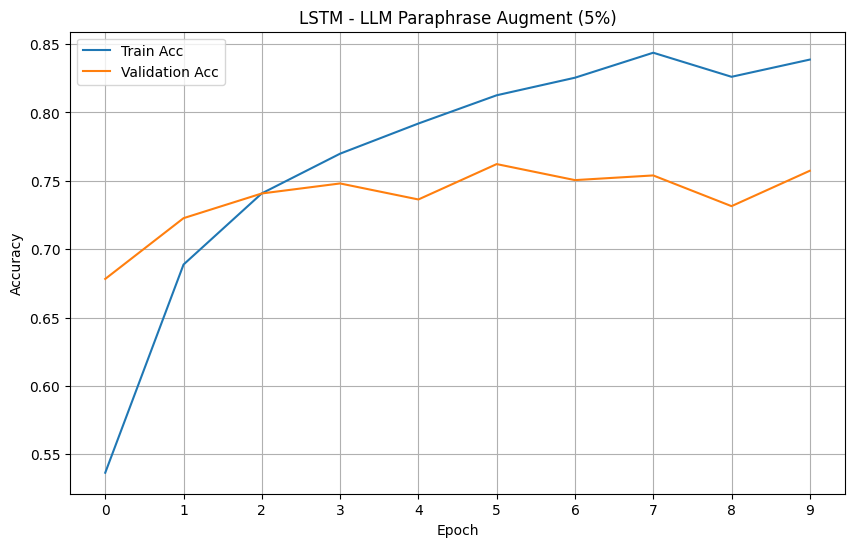
\includegraphics[width=\textwidth]{img/llm_5_lstm.png}
    \caption{5\% Augmentation}
    \label{fig:llm_5_lstm}
  \end{subfigure}
  \hfill
  \begin{subfigure}[b]{0.3\textwidth}
    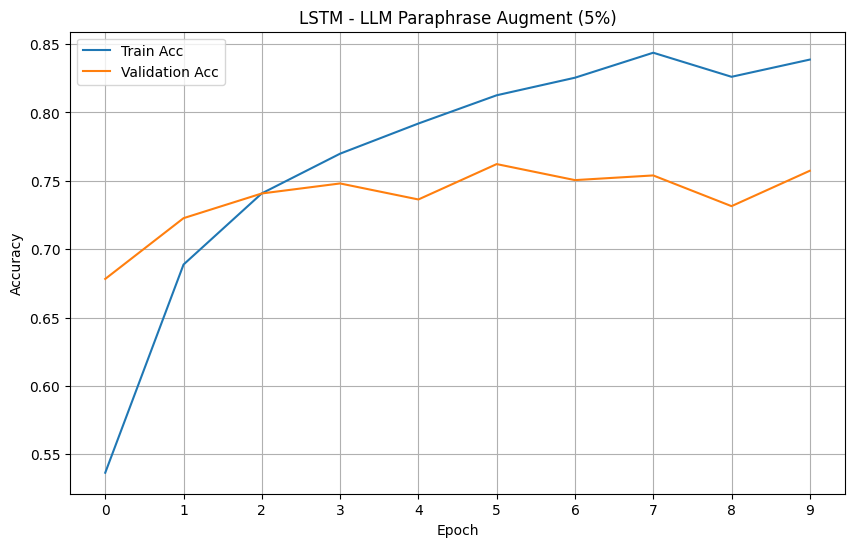
\includegraphics[width=\textwidth]{img/llm_10_lstm.png}
    \caption{10\% Augmentation}
    \label{fig:llm_10_lstm}
  \end{subfigure}
  \hfill
  \begin{subfigure}[b]{0.3\textwidth}
    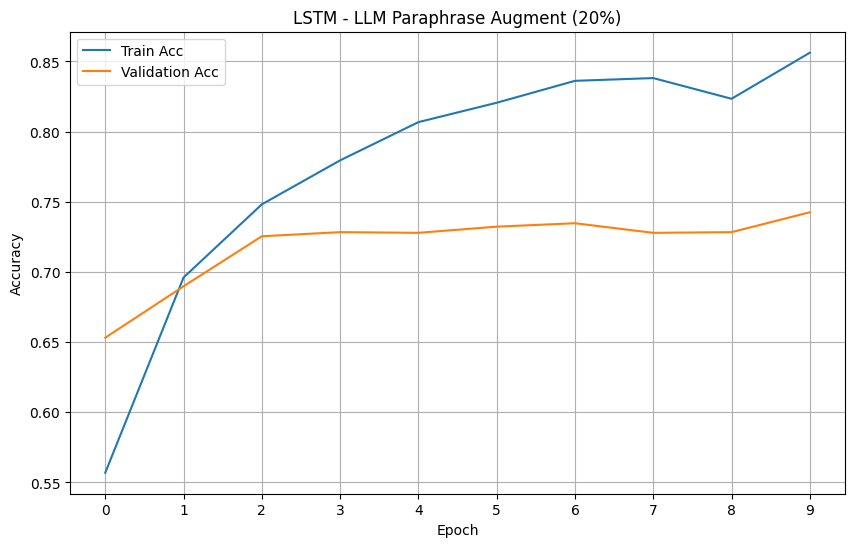
\includegraphics[width=\textwidth]{img/llm_20_lstm.png}
    \caption{20\% Augmentation}
    \label{fig:llm_20_lstm}
  \end{subfigure}
  \caption{Accuracy graphs for llm substitution DA at 5\%, 10\%, and 20\% levels on LSTM.}
  \label{fig:llm_lstm_substitution_accuracy}
\end{figure}

It is interesting to see that even on a more complex model, the performance
gain of augmentation through LLM is limited or worse than the rule-based
methods (Table \ref{fig:llm_lstm_substitution_accuracy}).

\begin{figure}[ht]
  \centering
  \begin{subfigure}[b]{0.45\textwidth}
    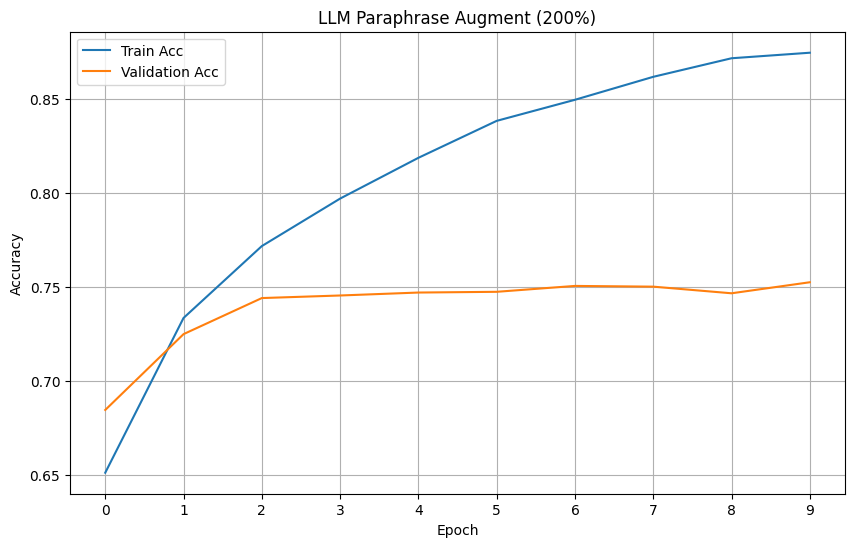
\includegraphics[width=\textwidth]{img/llm_200_rnn.png}
    \caption{200\% LLM Augmentation on RNN}
    \label{fig:llm_200_rnn}
  \end{subfigure}
  \hfill
  \begin{subfigure}[b]{0.45\textwidth}
    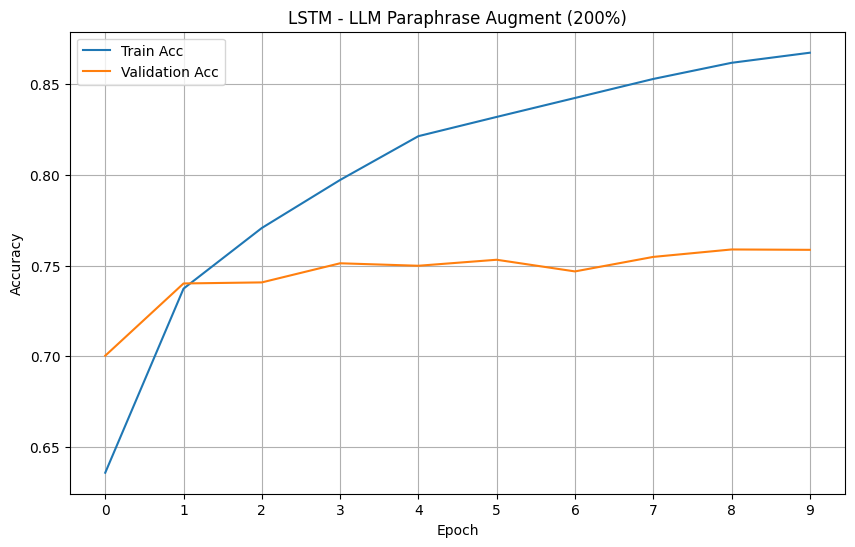
\includegraphics[width=\textwidth]{img/llm_200_lstm.png}
    \caption{200\% LLM Augmentation on LSTM}
    \label{fig:llm_200_lstm}
  \end{subfigure}
  \caption{Accuracy graphs on extreme LLM augmentation.}
  \label{fig:llm_extreme_substitution_acc}
\end{figure}

We can also see similar trends in the extreme cases of data augmentation in the
LLM setting as well. We further examined the potential causes and narrowed down
the issue to the following:

\begin{enumerate}
  \item The generated samples contained too many OOV that the model was not able to
        learn from. Our embedding layer only updates parameters for known words and
        does not learn from OOV words.
  \item The noise introduced by the LLM was too high that the model was not able to
        learn from the samples.
\end{enumerate}

To handle the first issue, an embedding layer that learns from OOV words and
updates its vocab could be used. The handling of the second issue is more
complex as it would require a more detailed prompt engineering to generate
samples that are more relevant. Instead of moving with that approach, we opted
to use a summarization model to generate the samples from the existing data.

\paragraph{Summarization Model}

The summarizer model performs almost the same as the LLM model in the previous
section. The performance of the model (Figure \ref{fig:llm_summerizer})
compared to the random and synonym techniques did not show a clear advantage
when augmentation is below 20\%. The performance gain only starts to show when
augmentation levels continued to increase. The summarizer model chosen is the
\textbf{facebook Bart} model.

\begin{figure}[ht]
  \centering
  \begin{subfigure}[b]{0.45\textwidth}
    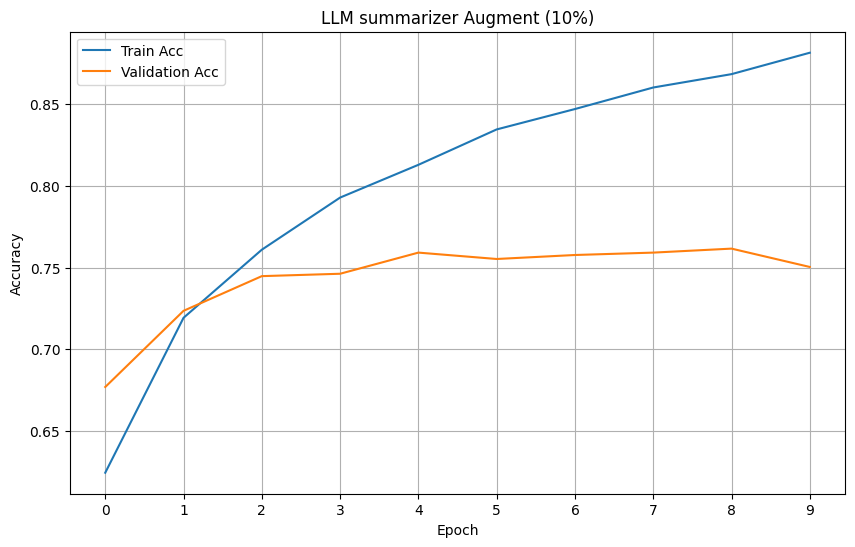
\includegraphics[width=\textwidth]{img/llm_summarise_10_rnn.png}
    \caption{10\% LLM (Summarize) Augmentation on RNN}
    \label{fig:llm_summarise_10_rnn}
  \end{subfigure}
  \hfill
  \begin{subfigure}[b]{0.45\textwidth}
    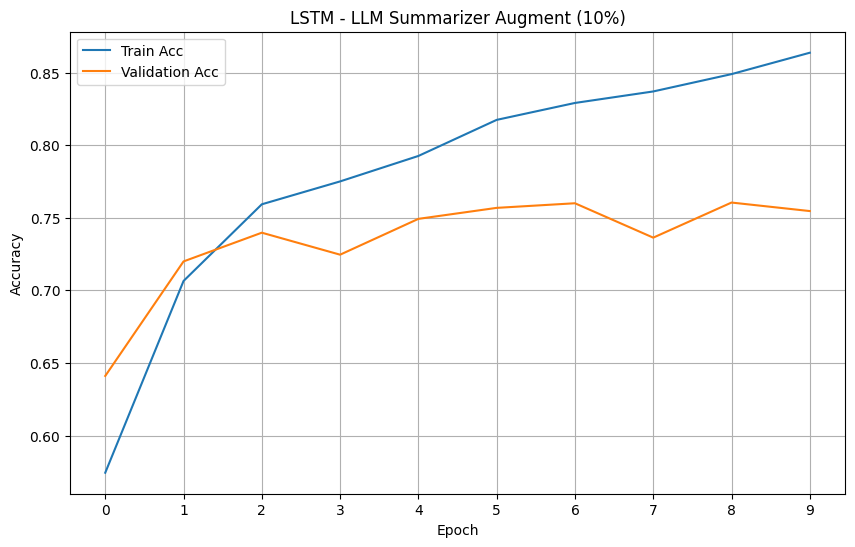
\includegraphics[width=\textwidth]{img/llm_summarise_10_lstm.png}
    \caption{10\% LLM (Summarize) Augmentation on LSTM}
    \label{fig:llm_summarise_10_lstm}
  \end{subfigure}
  \caption{Accuracy graphs on LLM (Summarize) augmentation.}
  \label{fig:llm_summerizer}
\end{figure}

With augmentation levels at 200\%, the performance of the model improved
significantly (Figure \ref{fig:llm_extreme_summerizer}). The levels of accuracy
of the models exceeded the performance of the rule-based methods by a huge
margin with the RNN model out performing over 90\% accuracy. The LSTM model
also performed well with over 87\% accuracy.

On investigation, we found that the use of summarizers to generate samples
produced less OOV counts allowing the model with a static vocab to learn from
the samples. We also hypothesize that unlike the task of paraphrasing, the
summarizer had better capabilities to capture the essence of the text and
generate relevant samples.

\begin{figure}[ht]
  \centering
  \begin{subfigure}[b]{0.45\textwidth}
    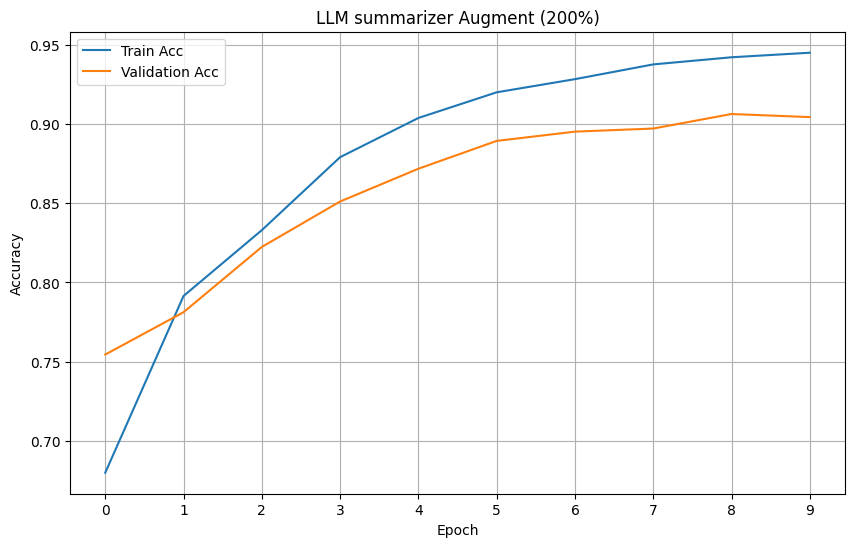
\includegraphics[width=\textwidth]{img/llm_summarise_200_rnn.png}
    \caption{200\% LLM (Summarize) Augmentation on RNN}
    \label{fig:llm_summarise_200_rnn}
  \end{subfigure}
  \hfill
  \begin{subfigure}[b]{0.45\textwidth}
    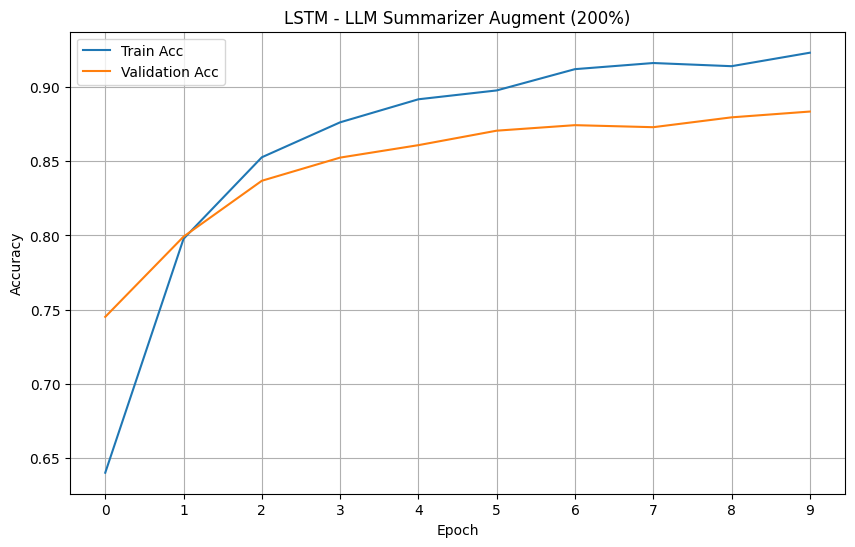
\includegraphics[width=\textwidth]{img/llm_summarise_200_lstm.png}
    \caption{200\% LLM (Summarize) Augmentation on LSTM}
    \label{fig:llm_summarise_200_lstm}
  \end{subfigure}
  \caption{Accuracy graphs on LLM (Summarize) extreme augmentation.}
  \label{fig:llm_extreme_summerizer}
\end{figure}

\section{NLarge: A Python Library for Data Augmentation}

We have developed a Python library called NLarge to DA for NLP sentiment
analysis. The library provides the methods and functions used in this report
along with models that can be used for sentiment analysis. The goal is to
provide a toolkit where users can easily experiment with different DA
techniques at various levels and models for sentiment analysis tasks. The
library can be accessed at \url{https://pypi.org/project/NLarge/} and the
source code is available at
\href{https://github.com/HiIAmTzeKean/SC4001-NLarge}{Github}.

We also made a website to provide end users with some information
\url{https://nlarge.com} such that we have an end to end solution for users. In
the website, we provide documentation on how to use the library and the
different methods that are available.

\begin{figure}[ht]
  \centering
  \begin{subfigure}[b]{0.45\textwidth}
    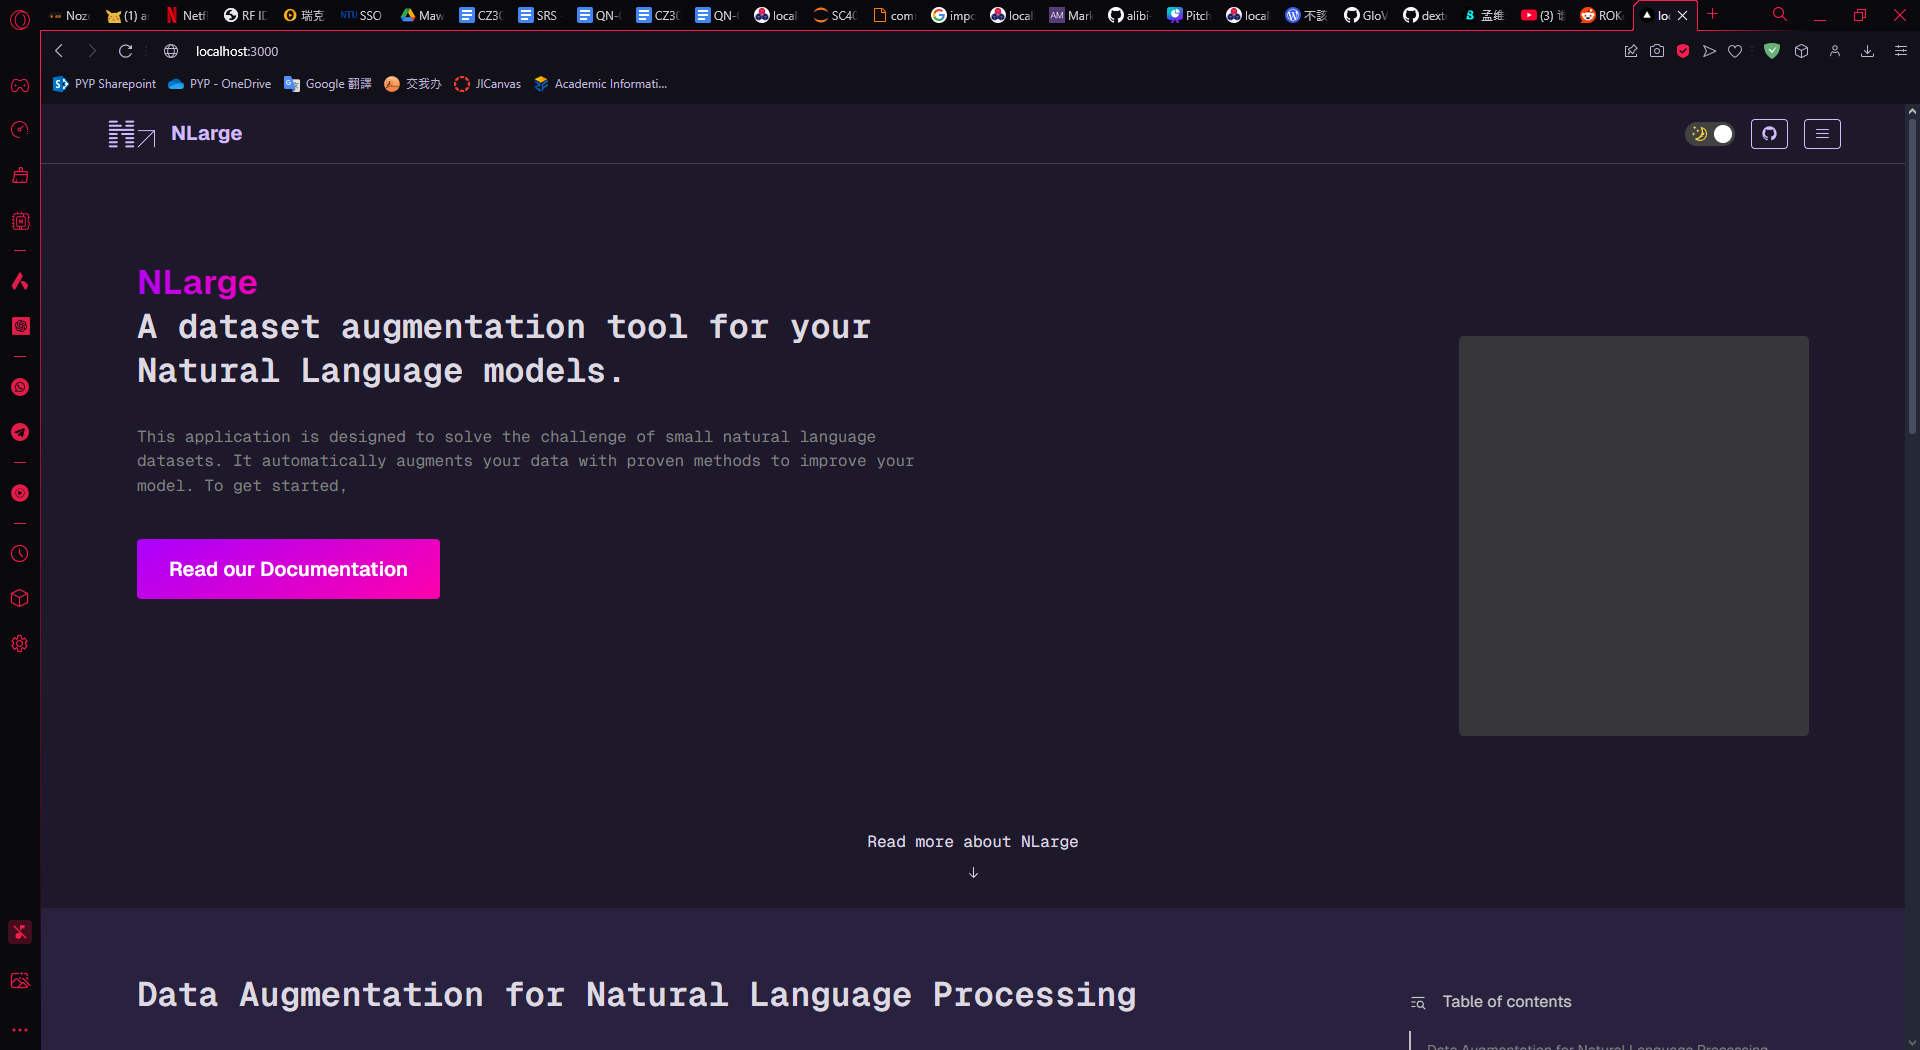
\includegraphics[width=\textwidth]{img/nlarge_web_1.png}
    \caption{Webpage Home}
    \label{fig:nlarge_web_1}
  \end{subfigure}
  \hfill
  \begin{subfigure}[b]{0.45\textwidth}
    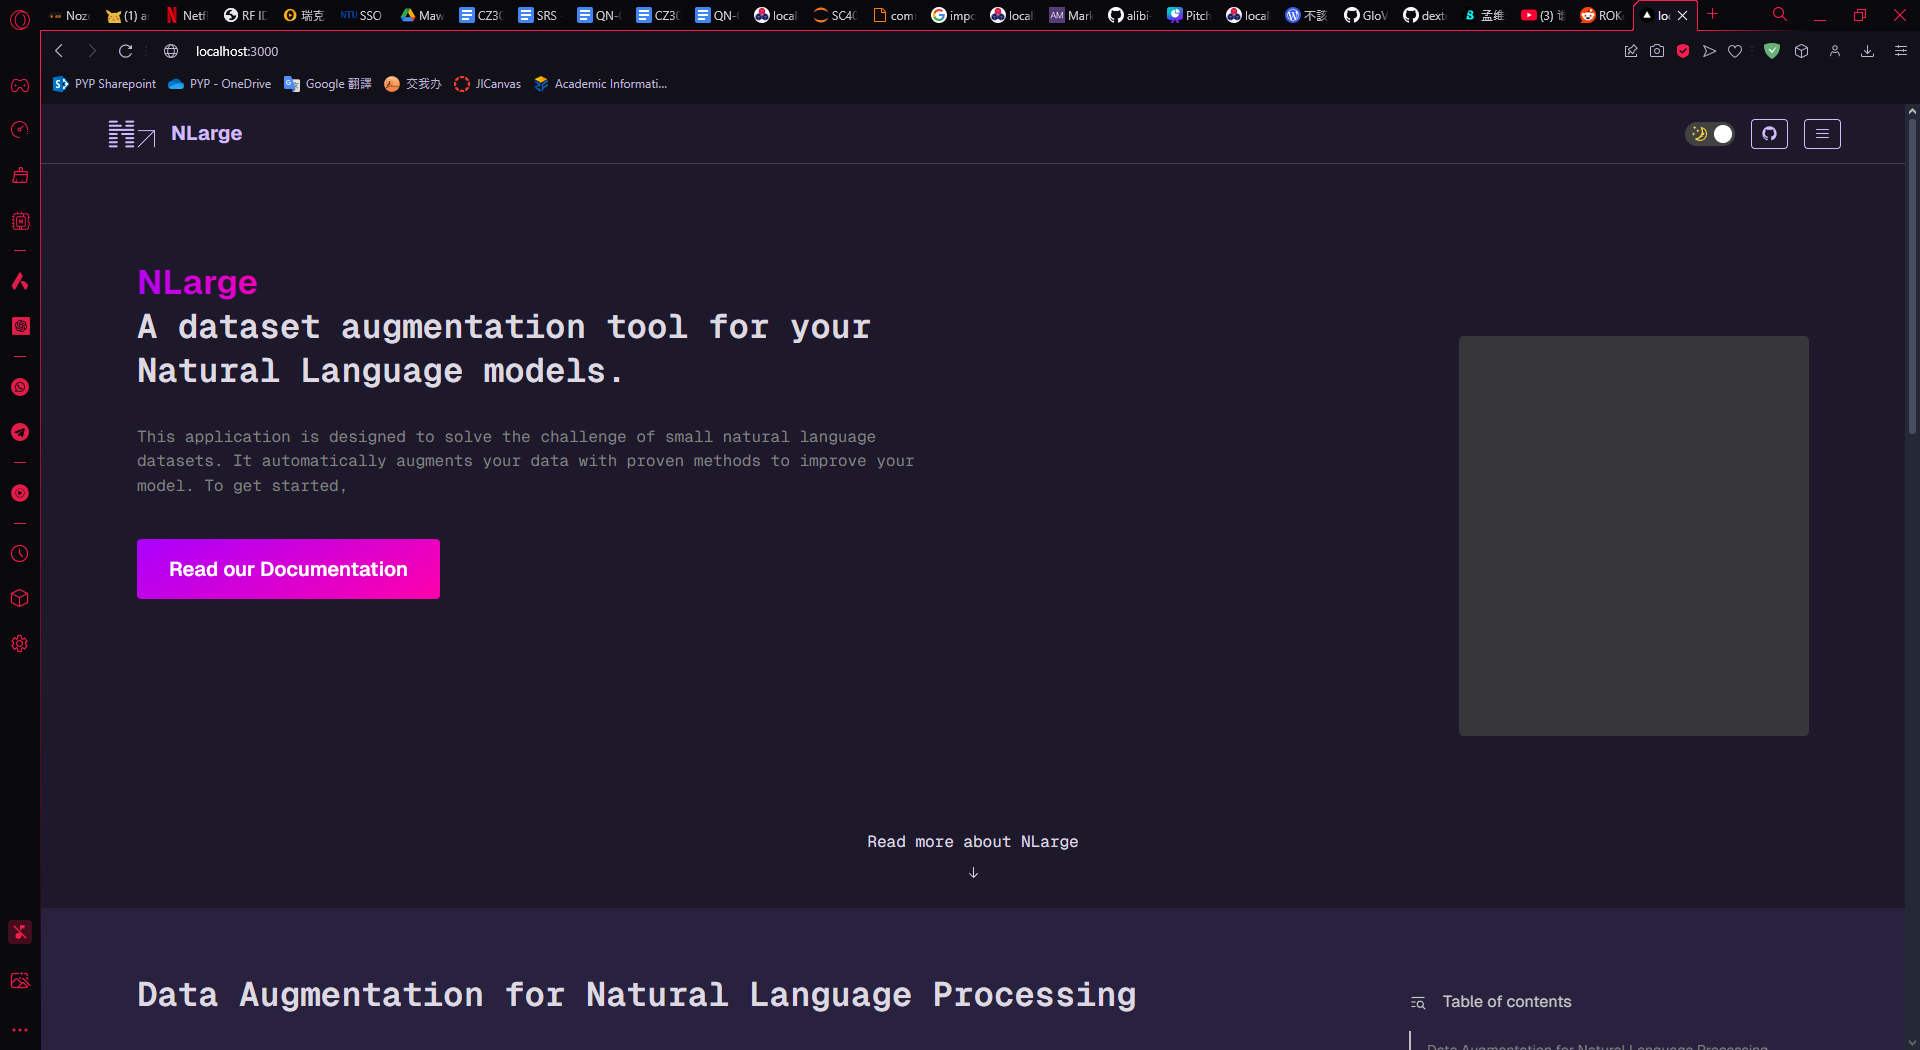
\includegraphics[width=\textwidth]{img/nlarge_web_1.png}
    \caption{Webpage Documentation}
    \label{fig:nlarge_web_2}
  \end{subfigure}
  \caption{NLarge website.}
  \label{fig:nlarge_web}
\end{figure}

\subsection{Discussion}

The experiments conducted in this study demonstrate the impact of DA techniques
on the performance of NLP models for sentiment analysis. Traditional methods
such as random substitution and synonym replacement provided a baseline
improvement in model performance by introducing variability into the training
data. However, these methods often fell short in capturing the nuanced
semantics and contextual dependencies inherent in natural language.

The introduction of advanced DA techniques using LLMs marked a substantial
improvement over traditional methods. Specifically, the use of LLMs for
summarization and paraphrasing generated high-quality augmented data that
significantly enhanced model performance. The results indicated that models
trained with LLM-augmented data achieved higher accuracy and better
generalization capabilities compared to those trained with traditional DA
methods.

The experiments with extreme augmentation levels (e.g., 200\%) further
highlighted the effectiveness of LLM-based DA. The RNN model, for instance,
achieved over 90\% accuracy, while the LSTM model reached over 87\% accuracy.
These findings suggest that LLMs can generate diverse and contextually relevant
samples that are beneficial for training robust NLP models.

One key observation was that the use of summarizers to generate augmented
samples resulted in fewer OOV counts. This allowed the models with a static
vocabulary to learn more effectively from the augmented data. Additionally,
summarizers were found to be more capable of capturing the essence of the text
and generating relevant samples compared to paraphrasing techniques.

Interestingly, the performance of the RNN model was generally better than that
of the LSTM model on the Rotten Tomatoes dataset. This can be attributed to
several factors. Firstly, the Rotten Tomatoes dataset consists of relatively
short text sequences, where the advantages of LSTM's ability to capture
long-term dependencies are less pronounced. RNNs, being simpler and less
computationally intensive, can perform well on such short sequences without the
overhead of managing long-term dependencies.

Secondly, LSTMs are designed to mitigate the vanishing gradient problem in long
sequences, but this advantage may not be fully utilized in datasets with
shorter text lengths. The additional complexity of LSTMs, including the gating
mechanisms, might introduce unnecessary overhead for short text sequences,
leading to slightly lower performance compared to RNNs.

We do note that the performance of the LSTM model was not superior to the RNN
when the token length of the LLM models were greater than 20 tokens because we
did not use a dynamically updating vocabulary size which could explain why in
this project, there was no clear advantage of the LSTM model.

We would also like to note that the task chosen at hand is specifically for
sentiment classification and that the findings in this report may not translate
to other tasks specific domains. However, we do believe that overall the use of
DA can potentially help in the case of over-fitting NLP tasks.

\subsection{Conclusion}

In conclusion, this study highlights the importance of data augmentation in
enhancing the performance of NLP models for sentiment analysis. Traditional DA
methods, while useful, have limitations in capturing the complexity of natural
language. Advanced techniques using LLMs, particularly for summarization and
paraphrasing, offer a promising solution by generating high-quality augmented
data that significantly improves model performance.

The development of the NLarge Python library provides a valuable toolkit for
researchers and practitioners to experiment with various DA techniques and
models for sentiment analysis. By offering a range of methods and functions,
NLarge aims to facilitate the exploration and implementation of effective DA
strategies in NLP tasks.

Future work could explore the integration of other advanced DA techniques and
further optimization of LLM-based methods. Additionally, expanding the library
to support a wider range of NLP tasks beyond sentiment analysis could provide
broader applicability and benefit to the NLP community.

Overall, the findings of this study underscore the potential of LLM-based data
augmentation to advance the state-of-the-art in NLP model performance and
generalization capabilities.

\bibliographystyle{plain}
\bibliography{bibliography.bib}

\end{document}